\subsubsection*{Ítem a}

\begin{figure}[H]
    \centering
    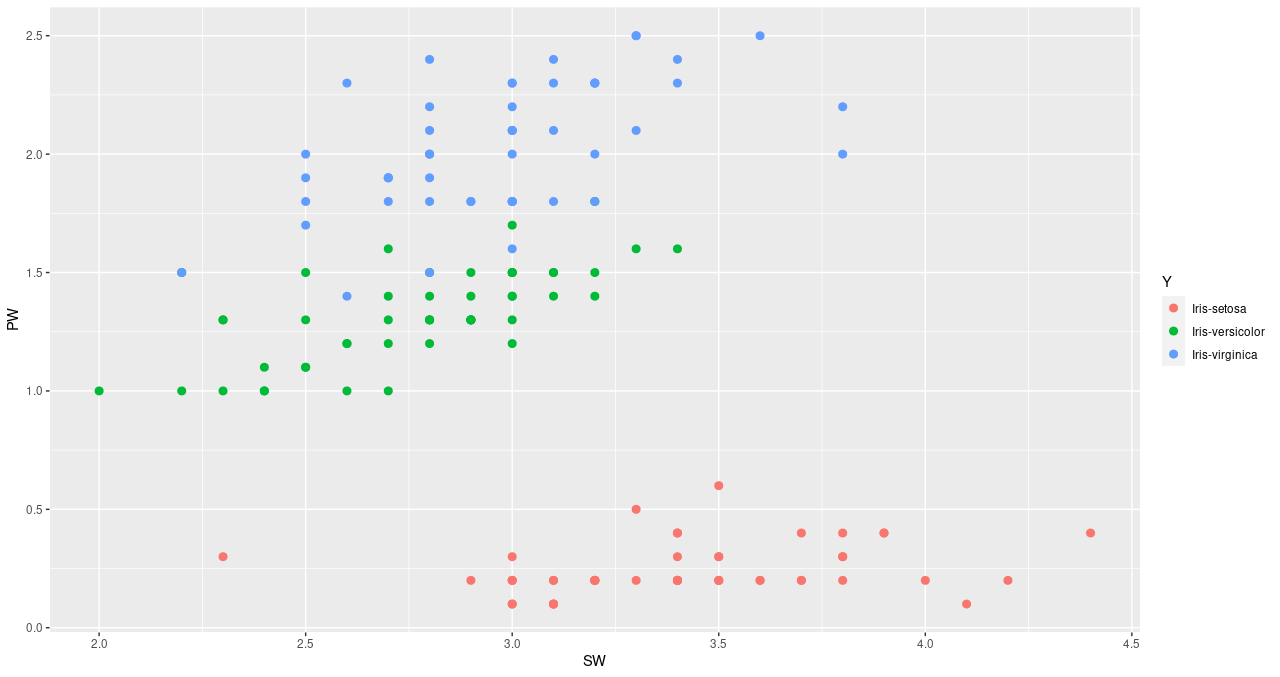
\includegraphics[width=1\textwidth]{resources/X2vsX4.png}
    \caption{Gráfico del ancho de sépalo vs ancho de pétalo}
\end{figure}

A priori no observamos anomalías en la distribución como para descartar que se distribuyen normalmente. Por lo que no descartamos la posibilidad, sin embargo cabe resaltar un par de aspectos que son inusuales, como por ejemplo que las variables toman valores discretos (Además se repiten muchos de ellos). Esto se puede deber a la precisión de la herramienta utilizada para medir. 

Este hecho se puede observar claramente en los gráficos qqnorm, para los cuales se presentan escalones de valores separados en $0.1$cm. 

\begin{figure}[H]
    \centering
    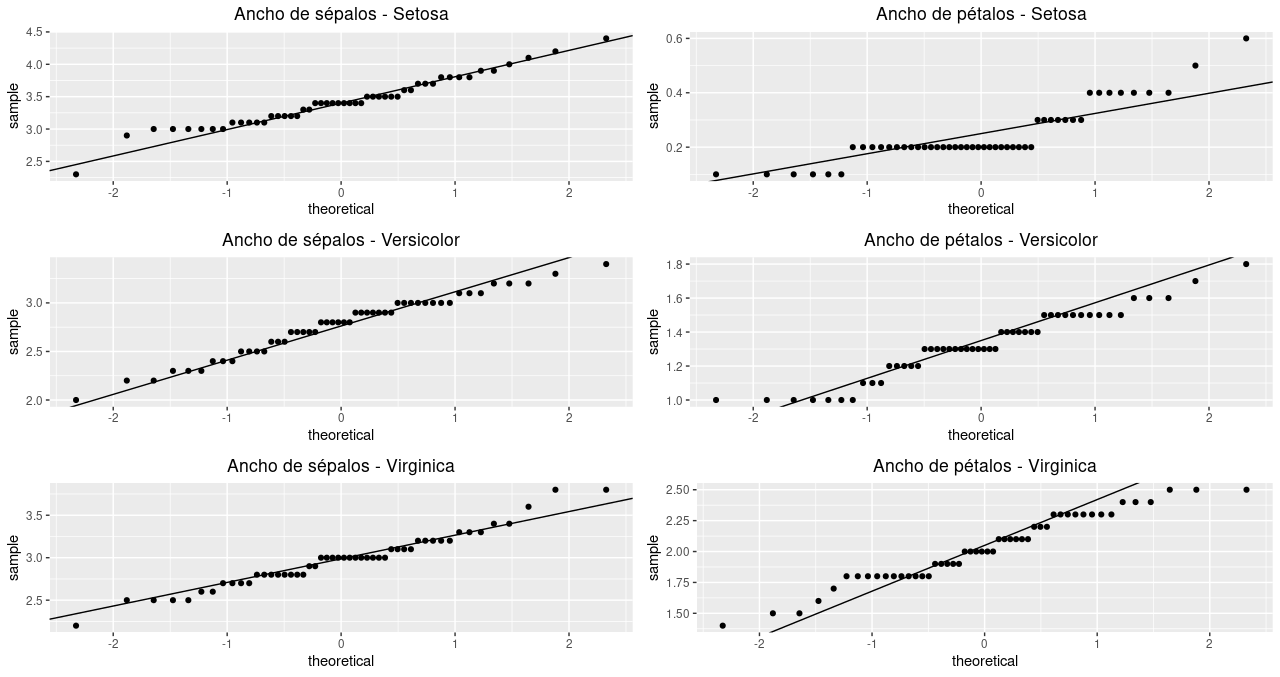
\includegraphics[width=1\textwidth]{resources/qqplots.png}
    \caption{Gráficos cuantil-cuantil por cada componente: comparación con normal}
\end{figure}

Podemos ver que si bien algunos gráficos dan idea de posible normalidad, otros son más delicados, como por ejemplo en gráfico de “Ancho de pétalos - Setosa” o el gráfico de “Ancho de pétalos - Virginica”.

\textbf{Ancho de pétalos - Setosa}


El gráfico de ancho de pétalos para Setosa tiene el problema previamente mencionado sobre la posible poca precisión de la herramienta utilizada, esto provoca en el gráfico que haya múltiples valores en sólo una capa y no un progreso continuo como es esperado para una distribución normal. Se puede observar el mismo fenómeno mencionado al realizar un experimento de distribución normal pero redondeada a sólo un decimal de significación:

\begin{figure}[H]
    \centering
    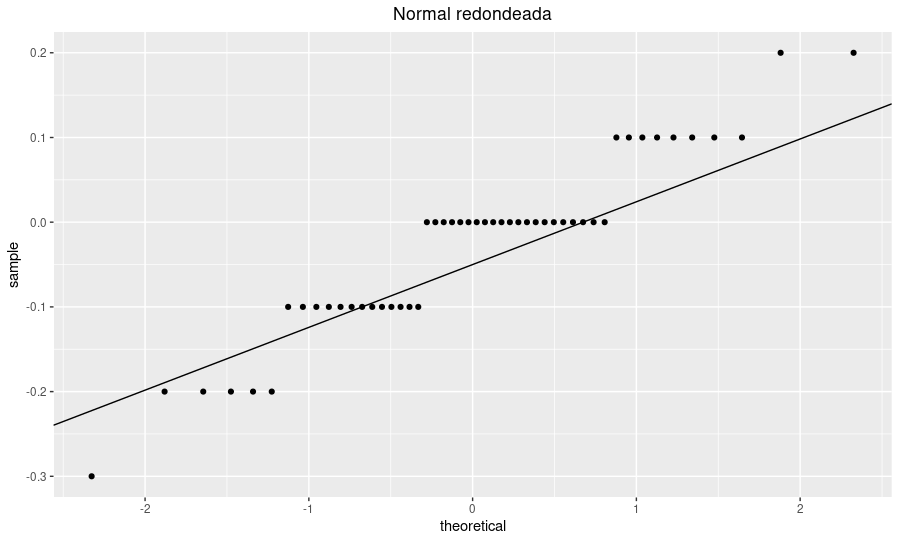
\includegraphics[width=0.6\textwidth]{resources/qqplot_roundnormal.png}
    \caption{Gráficos cuantil-cuantil para una distribución $\mathcal{N}(0; 0.1^2)$ redondeada}
\end{figure}

Se puede ver que la distribución de la normal redondeada (producto de una muestra de una distribución normal pero redondeada a sólo 1 decimal significativo) se comporta de forma similar a la obtenida para el ancho de pétalos en Setosa, por lo que a priori sigue siendo posible lo comentado previamente. Sin embargo también resaltar que a diferencia del gráfico obtenido para la normal redondeada (cuya distribución es simétrica) la distribución bajo estudio posee cierto grado de asimetría en los valores.

\textbf{Ancho de pétalos - Virginica}

El gráfico de ancho de pétalos para Virginica tiene el problema de colas pesadas, como se puede observar en los extremos del gráfico los cuantiles difieren mucho de los teóricos, esto resulta en una llamativa alerta contra la suposición de normalidad.


\subsubsection*{Ítem b}
Asignando los valores $1:$ Iris-Setosa, $2:$ Iris-Versicolor, $3:$ Iris-virginica. Se tiene:

\begin{minipage}{\linewidth}
  \centering
  \begin{minipage}{0.25\linewidth}
        \begin{align*}
            \mu_1 &= \begin{bmatrix}
            3.418 \\
            0.244
            \end{bmatrix}
        \end{align*}
  \end{minipage}
  \hspace{0.05\linewidth}
  \begin{minipage}{0.25\linewidth}
        \begin{align*}
            \mu_2 &= \begin{bmatrix}
            2.770 \\
            1.326
            \end{bmatrix}
        \end{align*}
  \end{minipage}
  \hspace{0.05\linewidth}
  \begin{minipage}{0.25\linewidth}
        \begin{align*}
            \mu_2 &= \begin{bmatrix}
            2.974 \\
            2.026
            \end{bmatrix}
        \end{align*}
  \end{minipage}
\end{minipage}

\vskip0.5cm

\begin{minipage}{\linewidth}
  \centering
  \begin{minipage}{0.25\linewidth}
        \begin{align*}
            \Sigma_1 &= \begin{bmatrix}
            0.1452 & 0.0114 \\
            0.0114 & 0.0115
            \end{bmatrix}
        \end{align*}
  \end{minipage}
  \hspace{0.05\linewidth}
  \begin{minipage}{0.25\linewidth}
        \begin{align*}
            \Sigma_2 &= \begin{bmatrix}
            0.0985 & 0.0412 \\
            0.0412 & 0.0391
            \end{bmatrix}
        \end{align*}
  \end{minipage}
  \hspace{0.05\linewidth}
  \begin{minipage}{0.25\linewidth}
        \begin{align*}
            \Sigma_3 &= \begin{bmatrix}
            0.1040 & 0.0476 \\
            0.0476 & 0.0754
            \end{bmatrix}
        \end{align*}
  \end{minipage}
\end{minipage}
\vskip0.5cm
Las reglas de clasificación serán entonces:
\vskip0.5cm
\begin{minipage}{\linewidth}
  \centering
  \begin{minipage}{0.25\linewidth}
  $$
    g_1 = A \cap B
  $$
  \end{minipage}
  \hspace{0.05\linewidth}
  \begin{minipage}{0.25\linewidth}
  $$
    g_2 = \overline{A} \cap C
  $$
  \end{minipage}
  \hspace{0.05\linewidth}
  \begin{minipage}{0.25\linewidth}
  $$
    g_3 = \overline{B} \cap \overline{C}
  $$
  \end{minipage}
\end{minipage}
\vskip0.5cm
siendo:

$$
    A = \{ X \in \mathbb{R}^{2}: 5.35x^{2} - 24.33y^{2} - 11.70xy - 1.20x - 10.02y - 0.499 > 0 \}
$$

$$
    B = \{ X \in \mathbb{R}^{2}: 3.03x^{2} - 37.88y^{2} - 1.10xy + 0.81x - 14.77y + 7.011 > 0\}
$$

$$
    C = \{ X \in \mathbb{R}^{2}: -2.32x^{2} - 13.54y^{2} + 10.6xy + 2.01x - 4.75y + 7.51 > 0\}
$$

Ahora, el valor $x_0 = (3.5 ; 1.75)$ cumple: 
\begin{itemize}
    \item $x_0 \in \overline{A}$
    \item $x_0 \in \overline{B}$
    \item $x_0 \in C$
\end{itemize}
Por lo tanto: $x_0 \in g_2$, y se clasificará como Iris-Versicolor.\\
Gráficamente:


\begin{figure}[H]
    \centering
    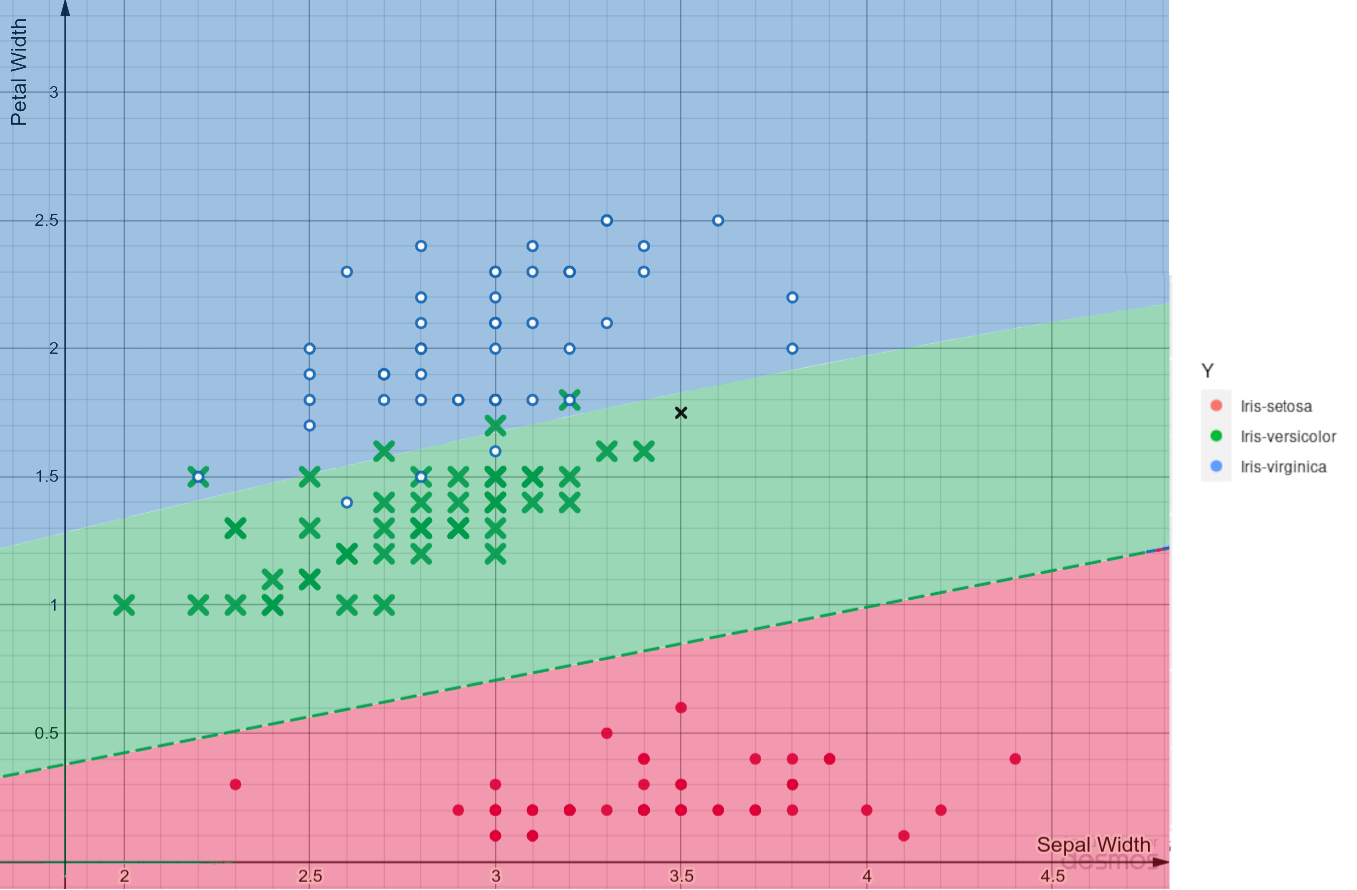
\includegraphics[width=1\textwidth]{resources/QDA_clasif.png}
    \caption{Clasificación cuadrática}
\end{figure}

Se pueden ver los valores correctamente clasificados, los incorrectamente clasificados y la cruz negra que muestra la posición de la nueva observación $x_0$.

\subsubsection*{Ítem c}
Dada la suposición de que las matrices de covarianza $\Sigma_i$ son iguales para cada población, utilizaremos la matriz $\Sigma$ que se calculará como:
$$
    \Sigma = \frac{1}{3}\Sigma_1 + \frac{1}{3}\Sigma_2 + \frac{1}{3}\Sigma_3
$$
Esto se debe a que, en la muestra, la probabilidad es igual para cada una de las clases.\\
Por lo que su valor será:
\begin{align*}
    \Sigma &= \begin{bmatrix}
    0.1159 & 0.0334 \\
    0.0334 & 0.0420
    \end{bmatrix}
\end{align*}
Por lo tanto las reglas de clasificacíon serán:
\vskip0.5cm
\begin{minipage}{\linewidth}
  \centering
  \begin{minipage}{0.25\linewidth}
  $$
    g_1 = A \cap B
  $$
  \end{minipage}
  \hspace{0.05\linewidth}
  \begin{minipage}{0.25\linewidth}
  $$
    g_2 = \overline{A} \cap C
  $$
  \end{minipage}
  \hspace{0.05\linewidth}
  \begin{minipage}{0.25\linewidth}
  $$
    g_3 = \overline{B} \cap \overline{C}
  $$
  \end{minipage}
\end{minipage}
\vskip0.5cm
siendo:

$$
    A = \{ X \in \mathbb{R}^{2}: 16.8973x - 39.1984y - 21.50952 > 0\}
$$

$$
    B = \{ X \in \mathbb{R}^{2}: 20.8495x - 59.0051y + 0.3357 > 0\}
$$

$$
    C = \{ X \in \mathbb{R}^{2}: 3.9522x-19.8067y+21.8452 > 0\}
$$

Ahora, el valor $x_0 = (3.5 ; 1.75)$ cumple: 
\begin{itemize}
    \item $x_0 \in \overline{A}$    
    \item $x_0 \in \overline{B}$
    \item $x_0 \in C$
\end{itemize}
Por lo tanto: $x_0 \in g_2$, y se clasificará como Iris-Versicolor.\\

Vale remarcar que al predecir al nuevo punto como Iris-Versicolor se está realizando una extrapolación en el ancho del sépalo. El dato con mayor ancho de sépalo de esta clase, tiene una menor longitud que el del nuevo registro a predecir. En consecuencia, no podemos afirmar que la predicción sea confiable.

Gráficamente:
\begin{figure}[H]
    \centering
    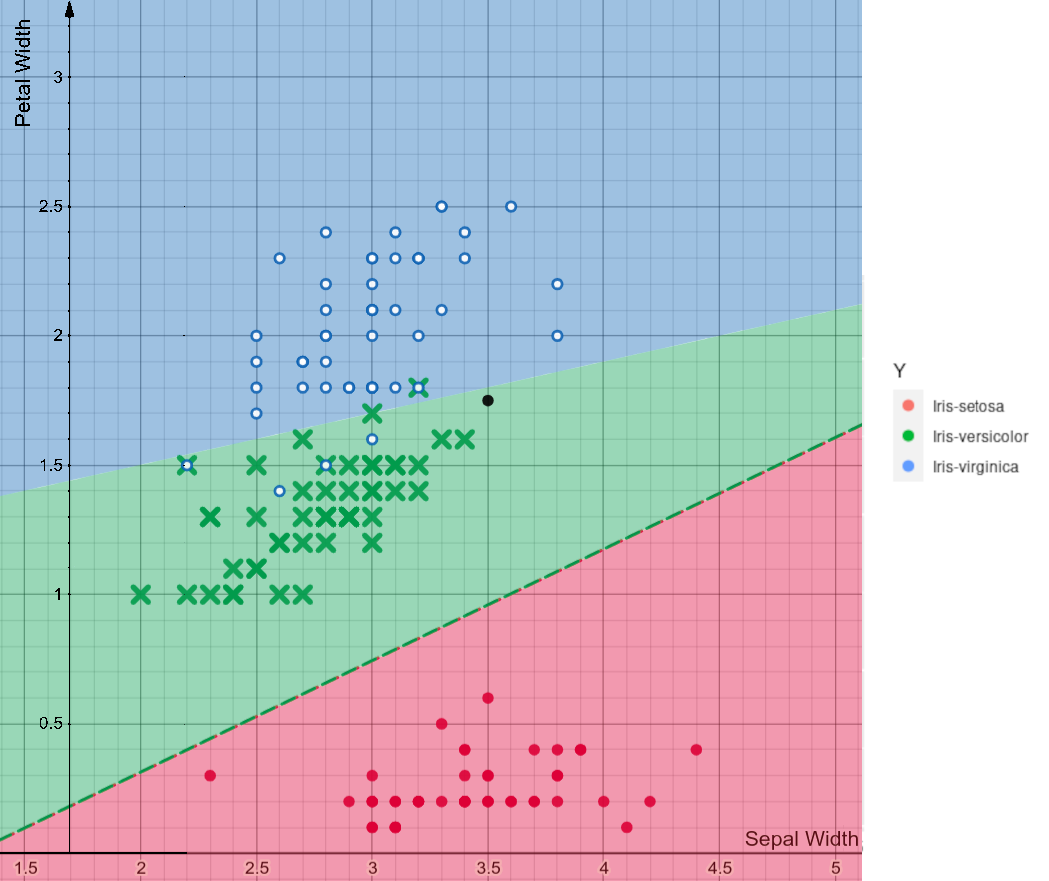
\includegraphics[width=1\textwidth]{resources/LDA_clasif.png}
    \caption{Clasificación lineal}
\end{figure}

Se pueden ver los valores correctamente clasificados, los incorrectamente clasificados y la cruz negra que muestra la posición de la nueva observación $x_0$.


\subsubsection*{Ítem e}

\textbf{LDA}
A continuación mostramos la matriz de confusión para LDA. De la misma se observa que el error aparente es de $5/150$

\begin{center}
    \begin{tabular}{|c|l|l|l|l|}
    \hline
    \multicolumn{2}{|l|}{\multirow{2}{*}{}}       & \multicolumn{3}{c|}{Clase predicha}            \\ \cline{3-5} 
    \multicolumn{2}{|l|}{}                        & Iris-setosa & Iris-versicolor & Iris-virginica \\ \hline
    \multirow{3}{*}{Clase real} & Iris-setosa     & 50          & 0               & 0              \\ \cline{2-5} 
                                & Iris-versicolor & 0           & 49              & 1              \\ \cline{2-5} 
                                & Iris-virginica  & 0           & 4               & 46             \\ \hline
    \end{tabular}
\end{center}

Utilizando el método de validación cruzada leave one out, se obtiene una estimación insesgada del error de $6/150$.

\textbf{QDA}

Por otro lado, para el caso de la regla de clasificación QDA obtuvimos la siguiente matriz de confusión, de la cual se puede observar un error aparente de $7/150$.
\begin{center}
    \begin{tabular}{|c|l|l|l|l|}
    \hline
    \multicolumn{2}{|l|}{\multirow{2}{*}{}}       & \multicolumn{3}{c|}{Clase predicha}            \\ \cline{3-5} 
    \multicolumn{2}{|l|}{}                        & Iris-setosa & Iris-versicolor & Iris-virginica \\ \hline
    \multirow{3}{*}{Clase real} & Iris-setosa     & 50          & 0               & 0              \\ \cline{2-5} 
                                & Iris-versicolor & 0           & 46              & 4              \\ \cline{2-5} 
                                & Iris-virginica  & 0           & 3               & 47             \\ \hline
    \end{tabular}
\end{center}

Se obtuvo por validación cruzada una estimación insesgada para el error de $8/150$. Nos llama particularmente la atención que el método de clasificación cuadrático (que dicho sea de paso, no asume matrices de covarianza idénticas) clasifique peor que el método de clasificación lineal.

